%\input{E:/Blaok/Works/LaTeX/MATLAB.tex}
\documentclass{article}
\usepackage{xeCJK}
\usepackage{indentfirst}
\usepackage{pifont}
\usepackage{graphicx}
\usepackage{listings}
\usepackage{xcolor}

\setmainfont{Georgia}
\setCJKmainfont{Source Han Sans SC}
\setCJKfamilyfont{kai}{KaiTi}
\setmonofont{Inconsolata}
\setlength{\parindent}{2em}
\setlength{\parskip}{1em}
\XeTeXlinebreaklocale "zh"
\XeTeXlinebreakskip = 0pt plus 1pt minus 0.1pt
\linespread{1}
\definecolor{codegreen}{rgb}{0,0.6,0}
\definecolor{codegray}{rgb}{0.5,0.5,0.5}
\definecolor{codepurple}{rgb}{0.58,0,0.82}
\lstset{
    captionpos=top,  
    commentstyle=\color{codegreen},
    keywordstyle=\color{blue},
    numberstyle=\tiny\color{codegray},
    stringstyle=\color{codepurple},
    breaklines=true,
    breakatwhitespace=false,
    frame=single,
    numbers=left,
    numberstyle=\tiny\color{gray},
    tabsize=4,
    title=\lstname,
    basicstyle=\ttfamily\footnotesize,
    language=Matlab
}







\begin{document}
\title{图像处理大作业}
\author{池雨泽}
\maketitle
\section{}
\subsection{}
\noindent\ding{125}{\CJKfamily{kai}MATLAB 提供了图像处理工具箱,在命令窗口输入 help images 可查看该工具箱内的所有函数。 请阅读并大致了解这些函数的基本功能。}\ding{126}
\par
感觉比较有用的函数有:imread/从文件读取图像、imwrite/写图像到文件、imshow/显示图像等。
\subsection{}
\noindent\ding{125}{\CJKfamily{kai}利用 MATLAB 提供的 Image file I/O 函数分别完成以下处理:\newline\indent(a) 以测试图像的中心为圆心,图像的长和宽中较小值的一半为半径画一个红颜色的圆:\newline\indent(b) 将测试图像涂成国际象棋状的“黑白格”的样子,其中“黑”即黑色,“白”则意味着保留原图。\newline 用一种看图软件浏览上述两个图,看是否达到了目标。}\ding{126}
\par 如下\begin{figure}\begin{center}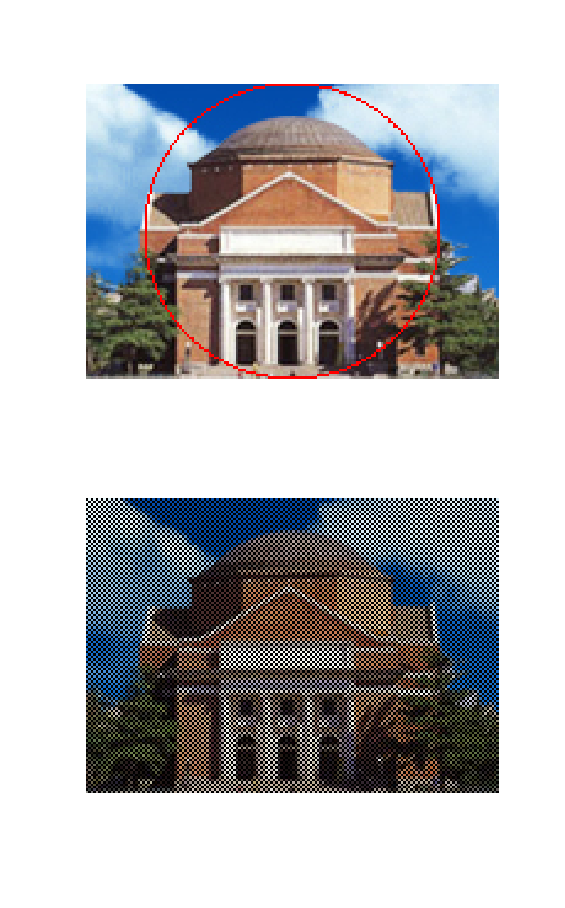
\includegraphics[width=\textwidth]{A3_1_2.eps}\end{center}\end{figure}
需要说明的是,这里我没有完全弄懂“国际象棋状的‘黑白格’的样子”到底应该是什么样,要是理解为$8\times8$的棋盘,那么每个格子便不是方形,与国际象棋棋盘不一致;如果保持每个格子为方形,那么又无法直观确定大小。最终,我决定选择以像素为单位染成黑白相见的格子。
\section{}
\subsection{}
\noindent\ding{125}{\CJKfamily{kai}图像的预处理是将每个像素灰度值减去 128 ,这个步骤是否可以在变换域进行?请在测试图像中截取一块验证你的结论。}\ding{126}
\par
是可以的。因为DCT是线性变换,减法和变换可以交换顺序。代码验证结果为有微小差异,应当是数值计算带来的误差。
\subsection{}
\noindent\ding{125}{\CJKfamily{kai}请编程实现二维 DCT ,并和 MATLAB 自带的库函数 dct2 比较是否一致。}\ding{126}
\par
从结果上看,二者完全一致。从代码上看,我实现的DCT是用脚本计算乘子矩阵实现,库函数则调用了两次dct函数,dct调用了内联的fft函数,因此虽然结果一致,自己写的dct\_2d性能远不如库函数。
\subsection{}
\noindent\ding{125}{\CJKfamily{kai}如果将 DCT 系数矩阵中右侧四列的系数全部置零,逆变换后的图像会发生什么变化?选取一块图验证你的结论。 如果左侧的四列置零呢?}\ding{126}
\par 
DCT系数右侧置零则图像只保留快速变化的整体部分,左侧置零则图像只保留缓慢变化的细节部分,如图所示。
\par\begin{center}\includegraphics[width=\textwidth]{A3_2_3.eps}\end{center}
\subsection{}
\noindent\ding{125}{\CJKfamily{kai}若对 DCT 系数分别做转置、 旋转 90 度和旋转 180 度操作 (rot90) ,逆变换后恢复的图像有何变化?选取一块图验证你的结论。}\ding{126}
\par 结果如下:转置使图像也被转置,沿主对角线被镜像;rot90以后出现横条纹,rot90两次以后出现网状的黑白相间条纹。转置没有改变图像高频和低频的信息,但由于关于对角线对称的点被对换,相应的位置信息也被对换,因而图像整体被转置。而旋转操作则混淆了高低频率的信息,高低频率信息对换,而图像本身低频分量高,对换放大了高频分量,产生了条状的条纹,两次旋转则使两个方向的条纹相对明显,产生网状花纹。
\par\begin{center}\includegraphics[width=\textwidth]{A3_2_4.eps}\end{center}


\subsection{}
\noindent\ding{125}{\CJKfamily{kai}如果认为差分编码是一个系统,请绘出这个系统的频率响应,说明它是一个\_\_\_\_(低通、 高通、 带通、带阻)滤波器。 DC 系数先进行差分编码再进行熵编码,说明 DC 系数的\_\_\_\_频率分量更多。}\ding{126}
\par 
差分无视低频分量,将高频分量放大通过,因此是高通滤波器。DC系数先差分再编码,说明低频分量多,差分可以压缩低频分量,节省编码空间。\par
差分编码的系统差分方程表示为$$y(n)=x(n-1)-x(n)$$系统函数为$$H(z)=-1+z^{-1}$$频率响应如下\par\begin{center}\includegraphics[width=\textwidth]{A3_2_5.eps}\end{center}

\subsection{}
\noindent\ding{125}{\CJKfamily{kai}DC 预测误差的取值和 Category 值有何关系?如何利用预测误差计算出其 Category ?}\ding{126}
\par Category取值取决于预测误差用二进制表示所需的最小位数。实际上,$$Category=\lceil\log_2(|\mbox{预测误差}|+1)\rceil$$

\subsection{}
\noindent\ding{125}{\CJKfamily{kai}你知道哪些实现 Zig-Zag 扫描的方法?请利用 MATLAB 的强大功能设计一种最佳方法。}\ding{126}
\par 实现Zig-Zag扫描,可以利用循环控制实现。一种思路是遍历矩阵,将每个元素置入对应的位置,难度在于元素矩阵坐标到矢量坐标的转换。一种思路是遍历矢量,将每个元素从对应的位置放入矢量,同样地,难点在于矢量坐标到矩阵坐标的转换。这两种算法优势在于,并行度高,可以通过并行计算提高效率,虽然在实际应用中可能并没有效果。简单而直观的思路是,按照扫描的顺序,依状态机的思路一个一个将矩阵元素装入矢量中,在矩阵中向左下或右上移动,到矩阵边缘则向右或向下移动一格,然后反向沿右上或左下方向移动,直到到达终点。由于这种方法计算量不大,简单易行,我采用了这种思路。

\subsection{}
\noindent\ding{125}{\CJKfamily{kai}对测试图像分块、 DCT 和量化,将量化后的系数写成矩阵的形式,其中每一列为一个块的 DCT 系数 Zig-Zag 扫描后形成的列矢量,第一行为各个块的 DC 系数。}\ding{126}
\par 
分块时要将不为8的整数倍的像素补齐。DCT使用了内置的函数。量化矩阵使用题给矩阵。zigzag函数为上一题的结果。最后得到一个64行的系数稀疏矩阵。

\subsection{}
\noindent\ding{125}{\CJKfamily{kai}请实现本章介绍的 JPEG 编码(不包括写 JFIF 文件),输出为 DC 系数的码流、 AC 系数的码流、图像高度和图像宽度,将这四个变量写入 jpegcodes.mat 文件。}\ding{126}
\par 编码程序使用函数jpegencode,输入为欲编码的图像灰度矩阵、DC码表、AC码表、量化步长矩阵,输出为DC码流、AC码流,还有编码的系数矩阵,以便与解码结果进行比较。\par 对于编码结果,由于是二进制流,我使用了logical型的行向量来存放。直流分量编码比较直观,扫一遍系数即可。交流分量编码我开始时使用了类似的思路,即扫描交流系数计算码流,但这样做有两个问题:一,效率低下,典型量化矩阵条件下,一般的照片交流分量比较稀疏,全部扫描浪费时间;二,处理EOB不方便,如果结尾0超过16个,需要判断不插入ZRL而直接插入EOB。于是我改为先查找系数中的非零部分,再扫描非零部分得到码流。

\subsection{}
\noindent\ding{125}{\CJKfamily{kai}计算压缩比(输入文件长度/输出码流长度),注意转换为相同进制。}\ding{126}
\par 我得到的压缩比为$6.4166$。这里,我认为输出码流长度应当计入图像大小信息。根据百度百科,jpeg格式支持uint16编码的图像大小,长和宽一共占用32位。

\subsection{}
\noindent\ding{125}{\CJKfamily{kai}请实现本章介绍的 JPEG 解码,输入是你生成的 jpegcodes.mat 文件。 分别用客观 (PSNR) 和主观方式评价编解码效果如何。}\ding{126}
\par 客观评价指标$PSNR=34.8926$。编码后解码的效果如图
\par 原图
\begin{center}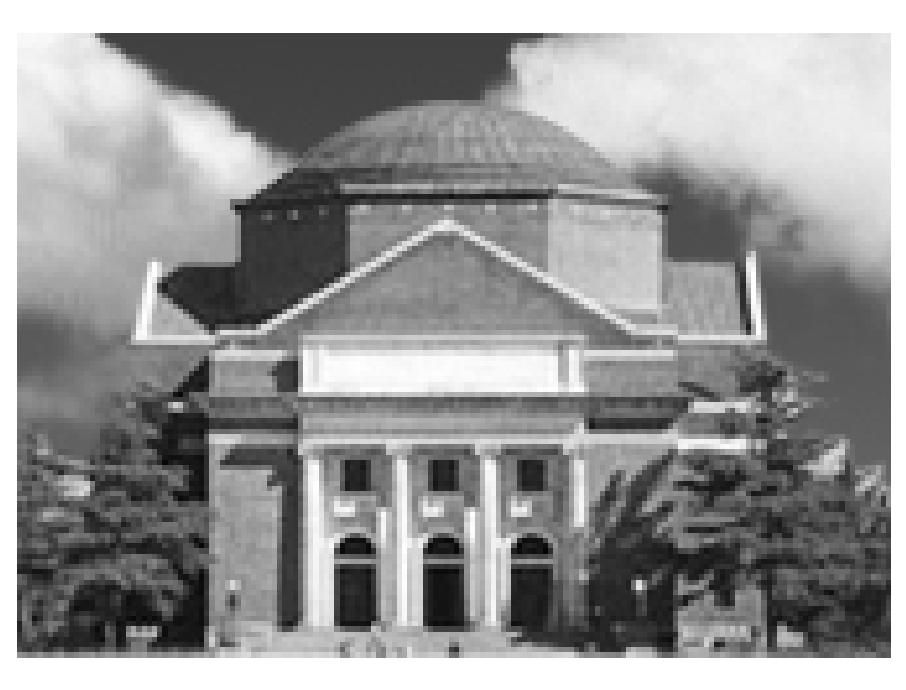
\includegraphics[width=\textwidth]{original.eps}\end{center}
\par 编码后解码的图
\begin{center}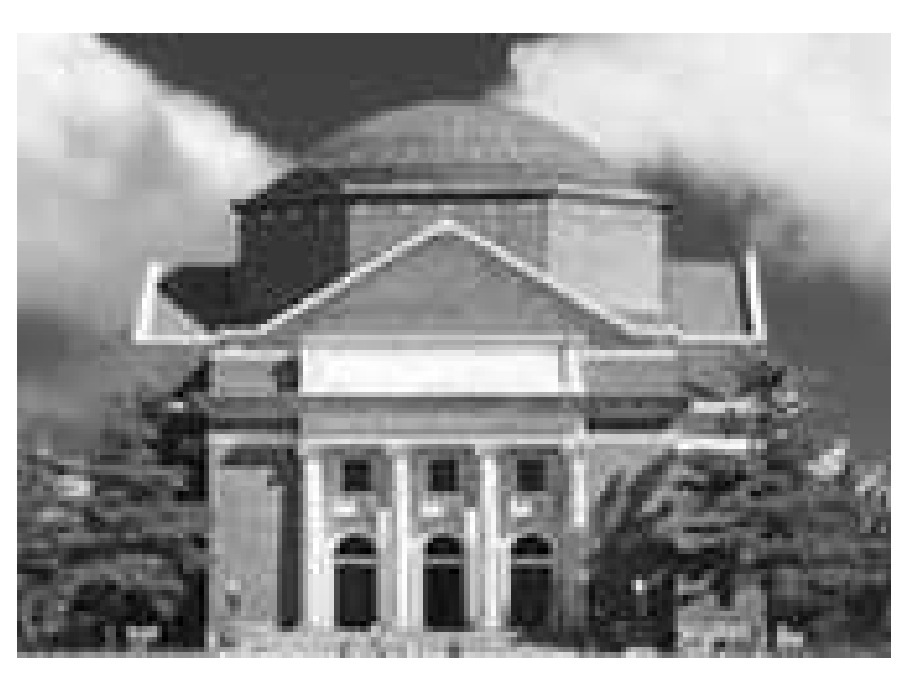
\includegraphics[width=\textwidth]{fullqtab.eps}\end{center}
\par 可见整体上没有明显的差异。细节上,JPEG编码明显使细节有所失真,在房屋的边缘出现原来没有的线条,这正是压缩高频分量导致的失真。

\subsection{}
\noindent\ding{125}{\CJKfamily{kai}将量化步长减小为原来的一半,重做编解码。 同标准量化步长的情况比较压缩比和图像质量。}\ding{126}
\par 使用一半的量化步长,得到压缩比为$4.4058$,$PSNR=37.3208$,可以看到图像细节上的失真有所减少,PSNR上升,但压缩比下降。
\par 使用一半量化步长编码后解码的图
\begin{center}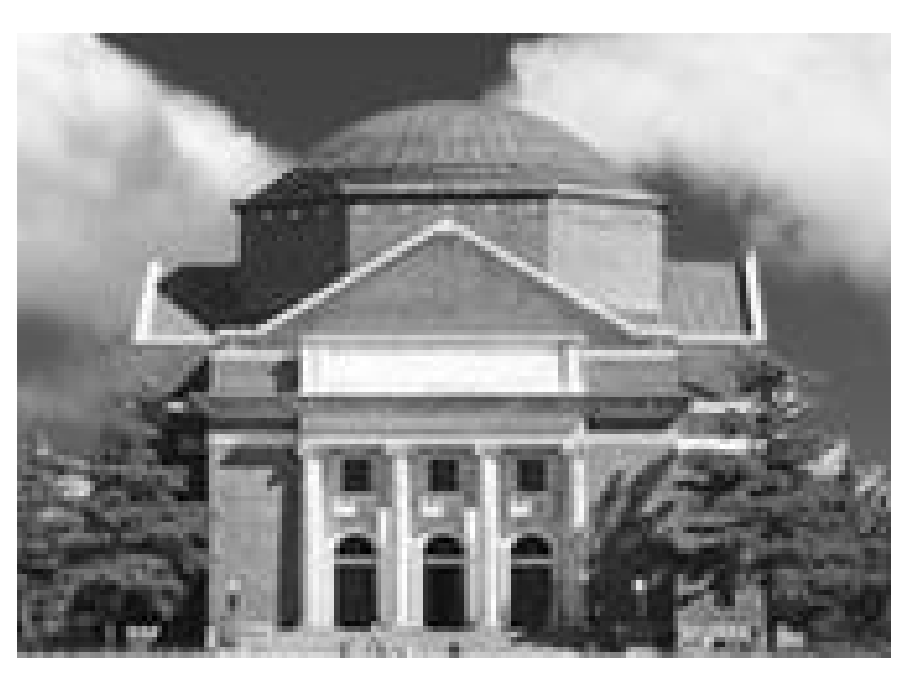
\includegraphics[width=\textwidth]{halfqtab.eps}\end{center}

\subsection{}
\noindent\ding{125}{\CJKfamily{kai}看电视时偶尔能看到美丽的雪花图像(见 snow.mat),请对其编解码。和测试图像的压缩比和图像质量进行比较,并解释比较结果。}\ding{126}
\par 雪花图像压缩比为$3.6564$,$PSNR=29.5614$。可以看出,雪花图像压缩比较低而图像质量却不高。这是因为,雪花图像中含有大量高频分量,难以较好地压缩。
\par 原图
\begin{center}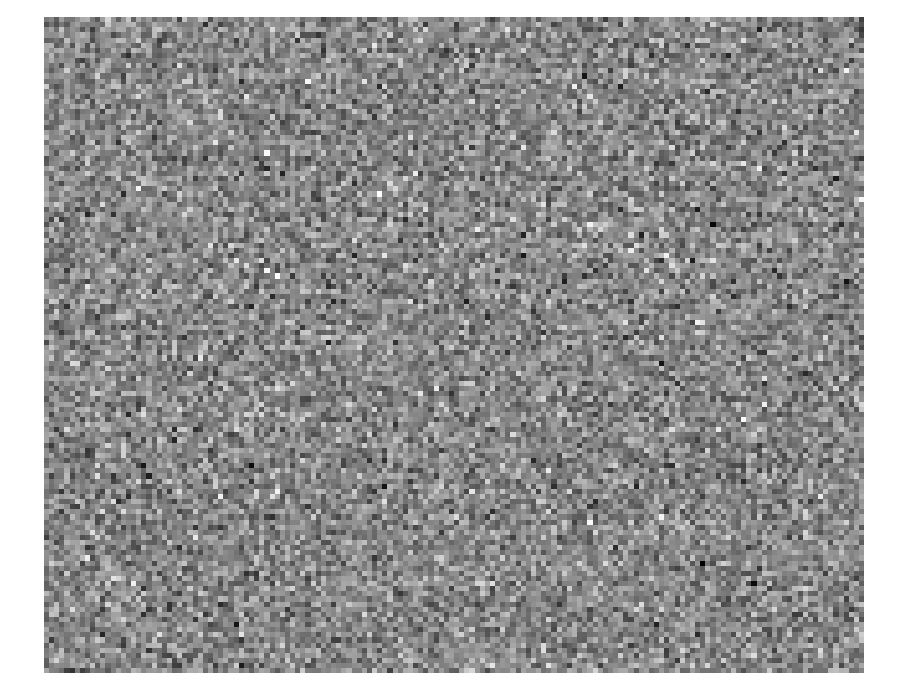
\includegraphics[width=\textwidth]{snow.eps}\end{center}
\par 压缩后的图
\begin{center}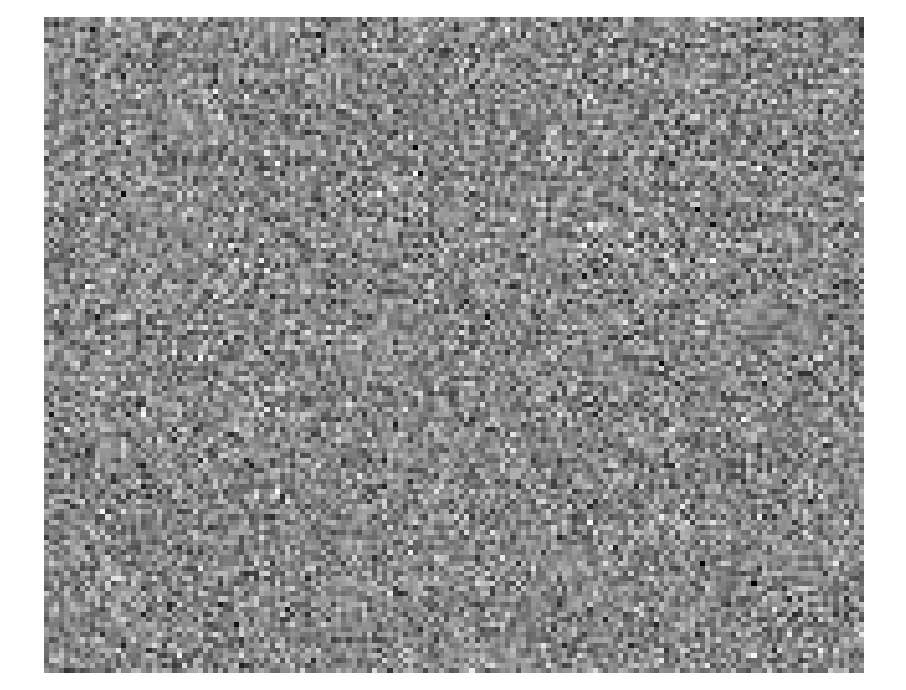
\includegraphics[width=\textwidth]{snow1.eps}\end{center}

\section{}
\subsection{}
\noindent\ding{125}{\CJKfamily{kai}实现本章介绍的空域隐藏方法和提取方法。 验证其抗 JPEG 编码能力。}\ding{126}
\par 空域隐藏后提取结果:
\par 	42 is the Answer to the Ultimate Question of Life, the Universe and Everything. This Answer was first calculated by the supercomputer Deep Thought after seven and a half million years of thought. This shocking answer resulted in the construction of an even larger supercomputer, named Earth, which was tasked with determining what the question was in the first place.
\par 出错位数: 0 (占0.00\%).
\par 空域隐藏并经过JPEG编解码后提取结果是一系列乱码。
\par 出错位数: 1472 (占50.14\%).
\par
\par 嵌入信息后的图
\begin{center}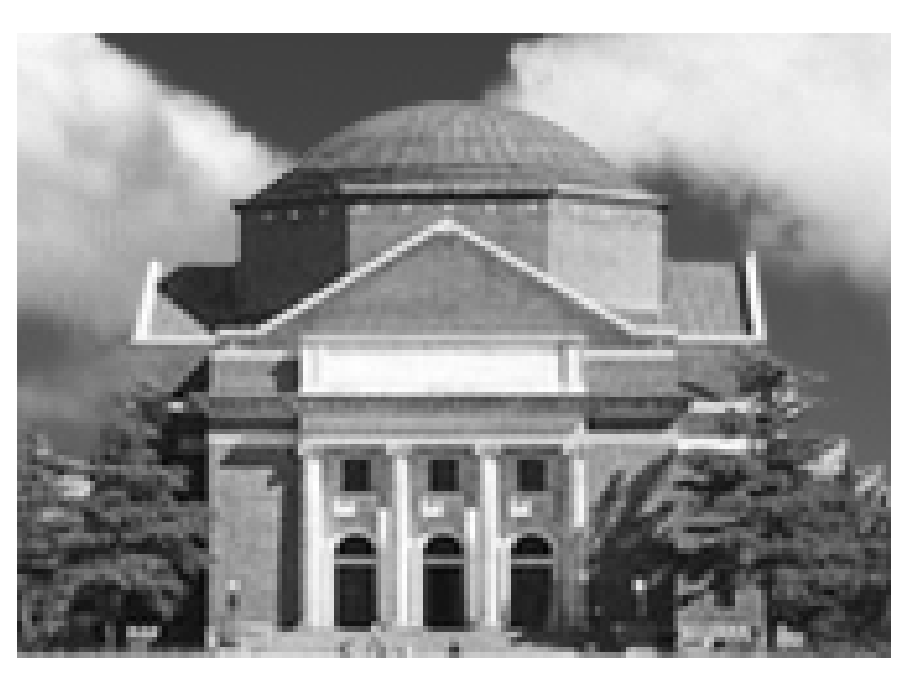
\includegraphics[width=\textwidth]{hidden0.eps}\end{center}
\par 可见,空域隐藏方法可以有效地嵌入隐藏信息,但不能抵抗JPEG编码。经过JPEG压缩之后,信息几乎全部丢失。这种方案对应的函数是imghide0和imgreveal0。

\subsection{}
\noindent\ding{125}{\CJKfamily{kai}依次实现本章介绍的三种变换域信息隐藏方法和提取方法,分析嵌密方法的隐蔽性以及嵌密后JPEG图像的质量变化和压缩比变化。}\ding{126}
\par 方法一提取结果:
\par 	42 is the Answer to the Ultimate Question of Life, the Universe and Everything. This Answer was first calculated by the supercomputer Deep Thought after seven and a half million years of thought. This shocking answer resulted in the construction of an even larger supercomputer, named Earth, which was tasked with determining what the question was in the first place.
\par 压缩率 6.2005; PSNR 33.22.
\par 嵌入信息后的图
\begin{center}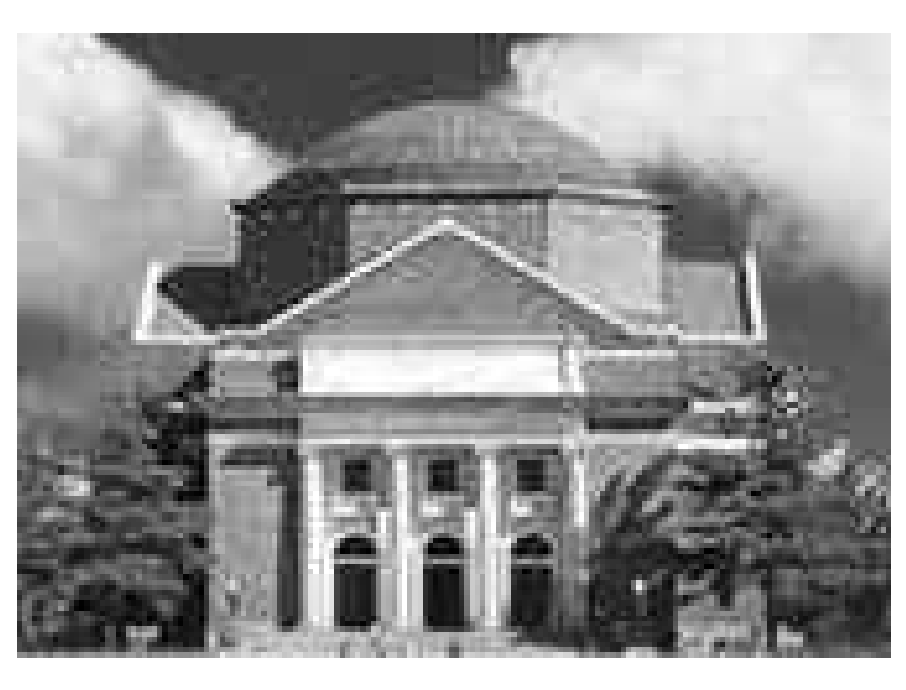
\includegraphics[width=\textwidth]{hidden1.eps}\end{center}
\par 方法二提取结果:
\par 	42 is the Answer to the Ultimate Question of Life, the Universe and Everything. This Answer was first calculated by the supercomputer Deep Thought after seven and a half million years of thought. This shocking
\par 压缩率 6.2682; PSNR 33.70.
\par 嵌入信息后的图
\begin{center}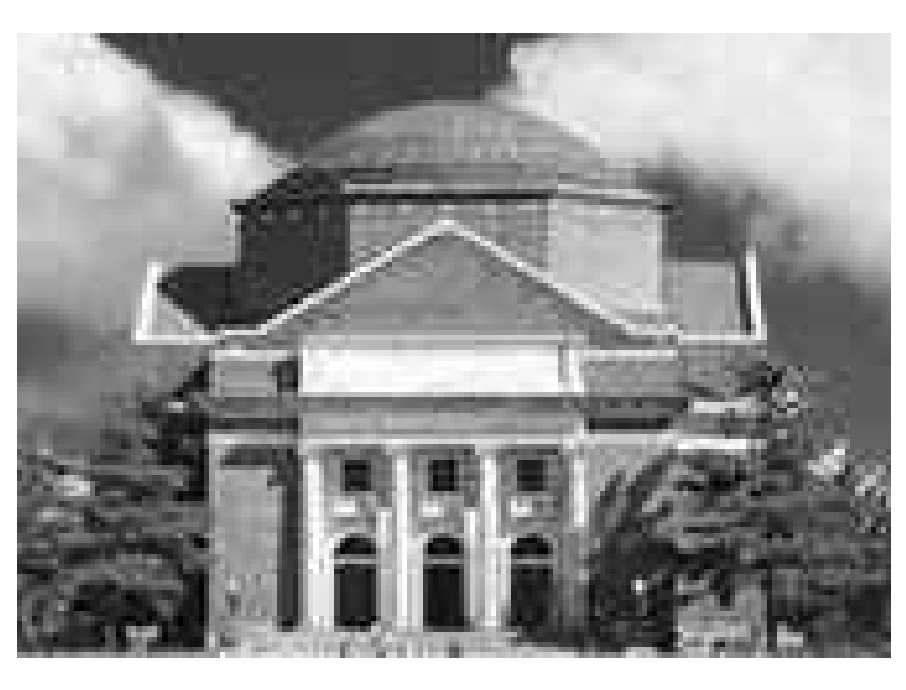
\includegraphics[width=\textwidth]{hidden2.eps}\end{center}
\par 方法三提取结果:
\par 	42 is t
\par 压缩率 6.1452; PSNR 33.17.
\par 嵌入信息后的图
\begin{center}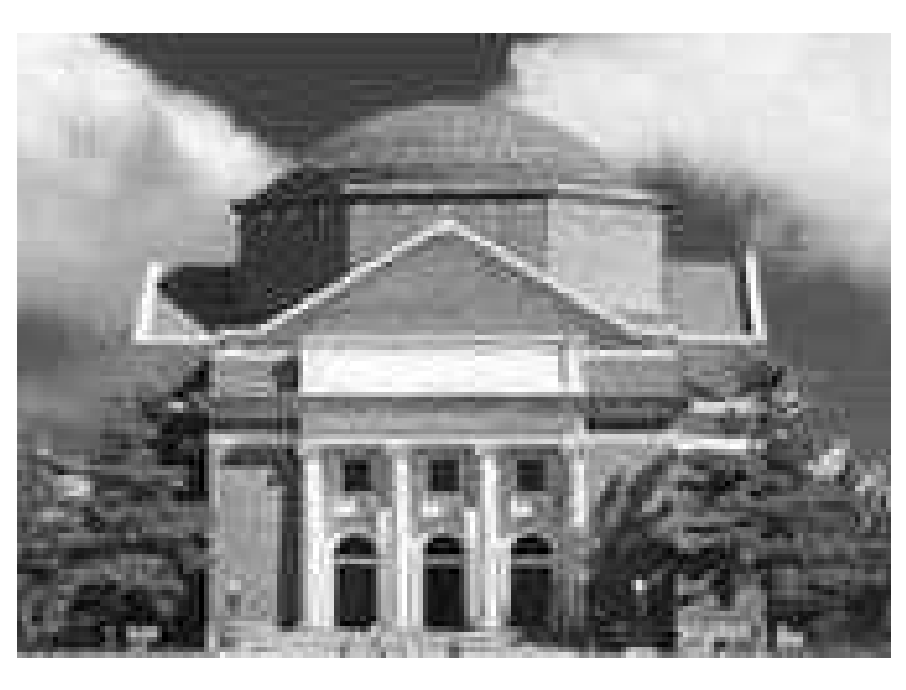
\includegraphics[width=\textwidth]{hidden3.eps}\end{center}
\par 算法中全都限制了嵌入信息的长度,也就是说信息过长时会自动计算可嵌入的信息长度嵌入。可见,相比空域嵌入方法,变换域信息隐藏方法可嵌入的信息量大大减少。隐蔽性方面,图像放大以后会有明显分块,特别是方法三。与正常照片明显不符,可以说隐蔽性均不理想。嵌入信息以后,从PSNR来看图像质量下降不大,但肉眼可以看出分块。压缩比方面,方法一和方法二令压缩比稍微下降,毕竟嵌入了信息。但实际上前两种方法不会改变系数的个数,因此不会对压缩比产生系统的影响,更不会有较大的偏差。第三种方法会添加系数,会较明显地降低压缩率,图像质量下降也因此较为显著。
\par 需要说明的是,题中没有明确说明前两个方法中被替换的系数是仅指非零系数还是将所有系数,包括零在内也算。我按前一种理解方式实现,因为如果将大量的零系数置为非零将明显影响图像质量,也影响压缩比。嵌入的信息饱和以后,会产生特别显著的花纹,造成隐蔽性下降。但仅替换非零系数也有一个问题,就是1可能被替换成0造成信息丢失。我的解决方法是,仅在大于1或小于0的系数中嵌入信息,即1不嵌入信息。
\par 方法一二三分别对应函数imghide[123]和imgreveal[123]。

\subsection{}
\noindent\ding{125}{\CJKfamily{kai}(选做)请设计实现新的隐藏算法并分析其优缺点。}\ding{126}
\par 方法四提取结果:
\par 	42 is the Answer to the Ultimate Question of Life, the Universe and Everything. This Answe
\par 压缩率 6.4163; PSNR 34.71.
\begin{center}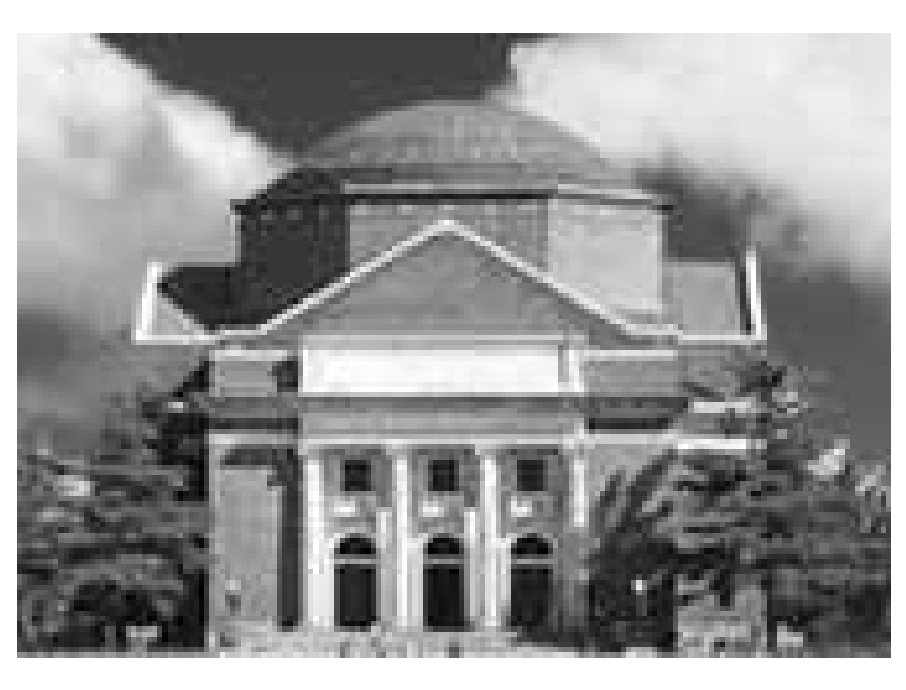
\includegraphics[width=\textwidth]{hidden4.eps}\end{center}
\par 我设计的方法是寻找DCT系数当中大于7或小于-6的系数在末位嵌入信息。这样,可以有效地保证原有信息被较好地保留,因为这些系数的绝对值较大,末位的改变不会明显改变它们的值。在编码质量和嵌密容量之间折衷,我最后选择的参数是>7或<-6。缺陷是,嵌入信息的能力较差,并且预先无法知道一定大小的图片可以嵌入的信息量。实际上,我认为比较理想的隐藏方法是直接在位图中末位嵌入信息,然后使用PNG等无损压缩格式来传输。为了保证隐蔽性,可以选择截图、绘图等一般不适于使用JPEG压缩的图形。
\par 对应函数imghide4和imgreveal4。

\section{}
\subsection{}
\noindent\ding{125}{\CJKfamily{kai}所给资料 Faces 目录下包含从网图中截取的 28 张人脸,试以其作为样本训练人脸标准 v 。\newline (a) 样本人脸大小不一,是否需要首先将图像调整为相同大小?\newline (b)  假设 L 分别取 3, 4, 5 ,所得三个 v 之间有何关系?}\ding{126}
\par 不需要调整大小,因为计算的是每张图中颜色所占的相对比例,与图片绝对大小无关。三个v的长度依次是前一个的8倍。

\subsection{}
\noindent\ding{125}{\CJKfamily{kai}设计一种从任意大小的图片中检测任意多张人脸的算法并编程实现(输出图像在判定为人脸的位置加 上红色的方框)。 随意选取一张多人照片(比如支部活动或者足球比赛),对程序进行测试。 尝试 L 分 别取不同的值,评价检测结果有何区别。}\ding{126}
\par 我的思路如下:先对图像进行分块,计算每一块与标准人脸之间的距离。寻找距离的最小值,初步认为这就是一张人脸。之后在附近一定范围内蛮力搜索不同位置和大小的图片部分,寻找其中距离最小的值作为人脸的结果。如果距离最小值超过某个阈值,就认定人脸已经全部找到。之所以用蛮力法搜索,是因为启发式算法在这里可能不稳定,因为颜色判断本身的鲁棒性并不好,会造成无法正确扩展寻找到合适的人脸,蛮力寻找虽然比较慢但一般可以找到合适的范围。最终结果如下
\par L=3
\begin{center}\includegraphics[width=\textwidth]{set1_1.eps}\end{center}
\par L=4
\begin{center}\includegraphics[width=\textwidth]{set1_2.eps}\end{center}
\par L=5
\begin{center}\includegraphics[width=\textwidth]{set1_3.eps}\end{center}
可以看出,三种L值都可以正确找出人脸位置,但细节上有一些不同;L=5时卡梅伦的手也被识别为人脸,但阈值降低则会有漏判,说明色彩直方图方法本身有一定缺陷,无法分辨颜色与人脸相近的其他图案。


\subsection{}
\noindent\ding{125}{\CJKfamily{kai}对上述图像分别进行如下处理后\newline
(a) 顺时针旋转 90◦ (imrotate):\newline
(b) 保持高度不变,宽度拉伸为原来的 2 倍 (imresize) :\newline
(c) 适当改变颜色 (imadjust) :\newline
再试试你的算法检测结果如何?并分析所得结果。}\ding{126}
\par 顺时针旋转九十度以后
\par L=3
\begin{center}\includegraphics[width=\textwidth]{set2_1.eps}\end{center}
\par L=4
\begin{center}\includegraphics[width=\textwidth]{set2_2.eps}\end{center}
\par L=5
\begin{center}\includegraphics[width=\textwidth]{set2_3.eps}\end{center}
\par 可以看出,旋转基本上不改变判断结果,仅卡梅伦的手误判增加。
\par 宽度拉伸以后
\par L=3
\begin{center}\includegraphics[width=\textwidth]{set3_1.eps}\end{center}
\par L=4
\begin{center}\includegraphics[width=\textwidth]{set3_2.eps}\end{center}
\par L=5
\begin{center}\includegraphics[width=\textwidth]{set3_3.eps}\end{center}
\par 结果仍可以接受。
\par 调整颜色以后(参数参照matlab help),就再也无法识别出人脸了。
\begin{center}\includegraphics[width=\textwidth]{set4.eps}\end{center}
\par 这说明,色彩直方图对于图像的旋转和拉伸不敏感,而对颜色极其敏感。这也是该方法最为不靠谱的地方,因为颜色被调整以后人眼仍可以轻易识别出人脸,但颜色直方图就不行,它丢弃了太多信息。

\subsection{}
\noindent\ding{125}{\CJKfamily{kai}如果可以重新选择人脸样本训练标准,你觉得应该如何选取?}\ding{126}
\par 我觉得要注意以下两点:一,注意有针对性地选择样本,样本与被测试对象越接近,正确判别的机会越大。这包括选择相近肤色、相近光照、相似方向的样本照片。二,注意对样本进行处理,去掉样本中边缘的杂乱色彩,使样本比较真实地反映肤色。对于题给的31个样本,我觉得其中有一些就可能造成样本带来较大偏差,例如9和24的阴影明显较多,大部分样本边缘都有黑边等等。如果可能,应当提取中间有代表性的部分作为采样区域。


\XeTeXdefaultencoding GBK
\lstinputlisting{A3_1_2.m}
\lstinputlisting{A3_2_1.m}
\lstinputlisting{A3_2_2.m}
\lstinputlisting{dct_2d.m}
\lstinputlisting{A3_2_3.m}
\lstinputlisting{A3_2_4.m}
\lstinputlisting{A3_2_5.m}
\lstinputlisting{A3_2_7.m}
\lstinputlisting{zigzag.m}
\lstinputlisting{izigzag.m}
\lstinputlisting{A3_2_8.m}
\lstinputlisting{A3_2_9.m}
\lstinputlisting{jpegencode.m}
\lstinputlisting{A3_2_a.m}
\lstinputlisting{A3_2_b.m}
\lstinputlisting{jpegdecode.m}
\lstinputlisting{A3_2_c.m}
\lstinputlisting{A3_2_d.m}
\lstinputlisting{A3_3_1.m}
\lstinputlisting{imghide0.m}
\lstinputlisting{imgreveal0.m}
\lstinputlisting{A3_3_2.m}
\lstinputlisting{imghide1.m}
\lstinputlisting{imgreveal1.m}
\lstinputlisting{imghide2.m}
\lstinputlisting{imgreveal2.m}
\lstinputlisting{imghide3.m}
\lstinputlisting{imgreveal3.m}
\lstinputlisting{A3_3_3.m}
\lstinputlisting{imghide4.m}
\lstinputlisting{imgreveal4.m}
\lstinputlisting{A3_4_1.m}
\lstinputlisting{A3_4_2.m}
\lstinputlisting{A3_4_3.m}
\XeTeXdefaultencoding auto
\end{document}
